\begin{figure}[ht]
\vskip 0.2in
\begin{center}
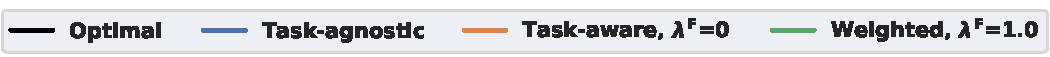
\includegraphics[width=0.8\columnwidth]{figures/evolution_legend.pdf}

\subfigure{
{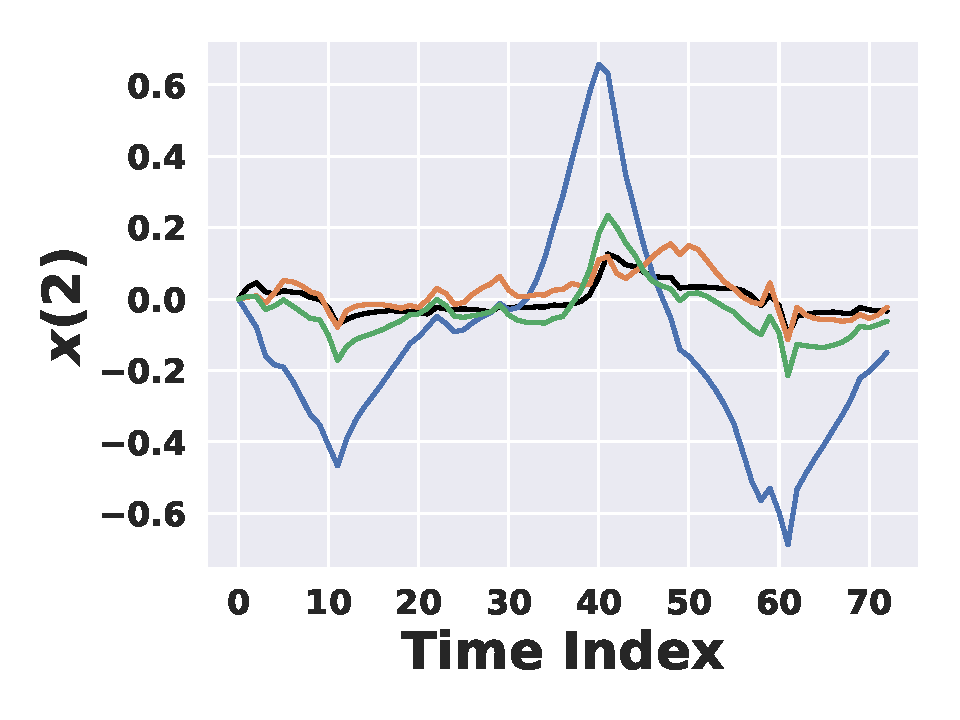
\includegraphics[width=0.31\columnwidth]{figures/appendix/iot/z_4/state_evolution_sample_1_state_2.pdf}}
\label{fig_synthetic_state_evolution}
}
\subfigure{
{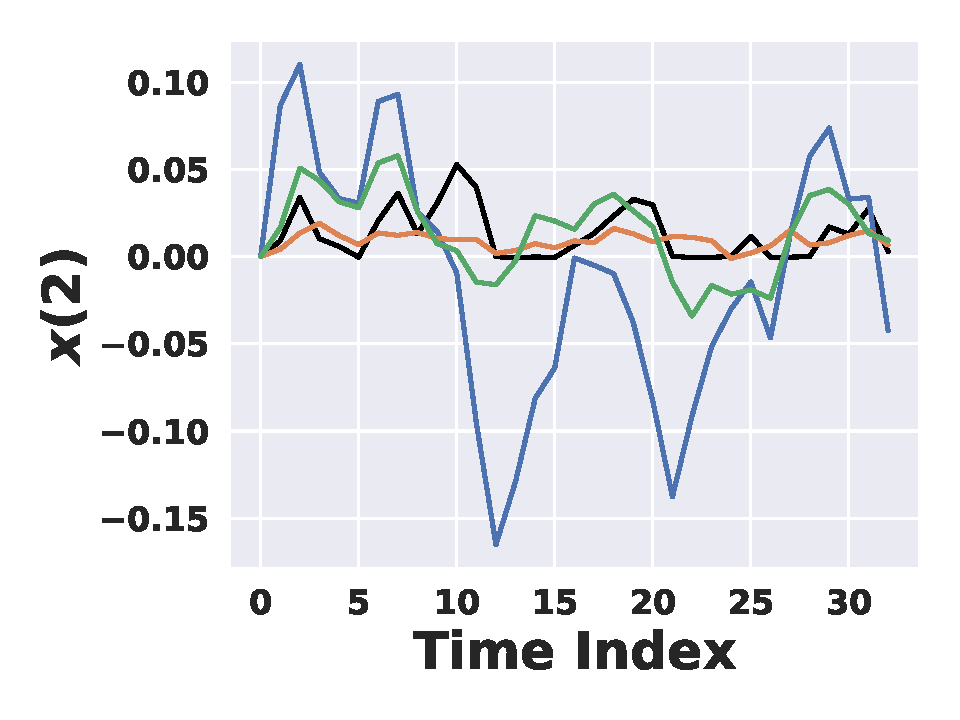
\includegraphics[width=0.31\columnwidth]{figures/appendix/cell/z_4/state_evolution_sample_1_state_2.pdf}}
}
\subfigure{
{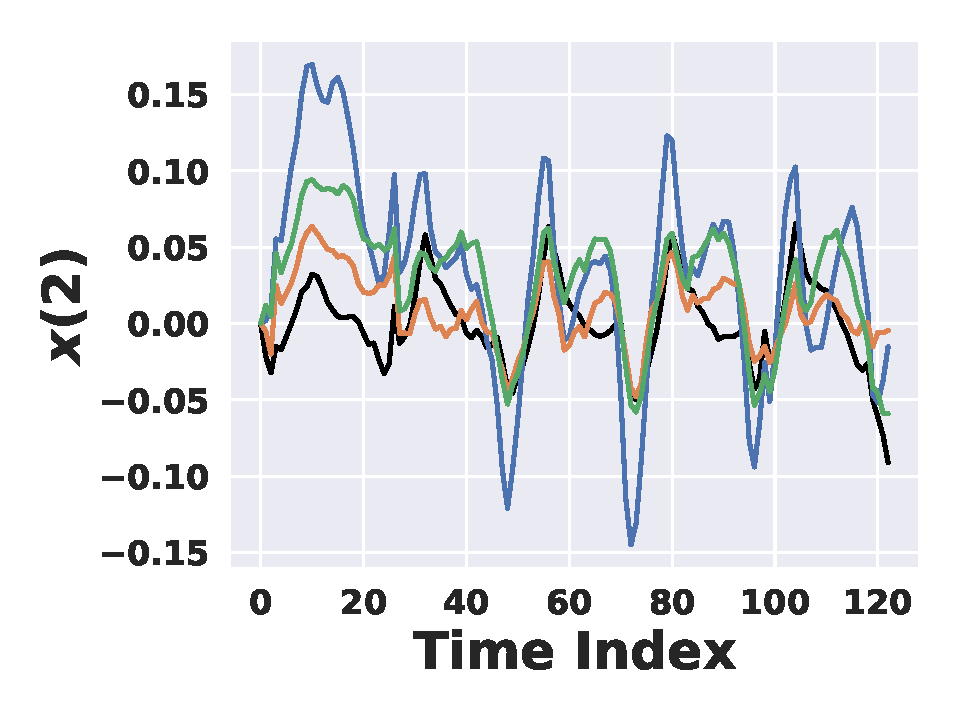
\includegraphics[width=0.31\columnwidth]{figures/appendix/pjm/z_4/state_evolution_sample_1_state_2.pdf}}
\label{fig_synthetic_forecast_errors}
}

\caption{Example evolution of $x(2)$ when $Z = 4$, for IoT (top), taxi scheduling (middle) and battery charging (bottom) scenarios, respectively. Clearly, our co-design approach has state evolutions closer to the unrealizable optimal solution (black) which assumes \textit{perfect} forecasts.}
\label{fig:state_evolution}
\end{center}
\vskip -0.2in
\end{figure}
